\chapter{Useful Probability Distribution}

\begin{itemize}
  \item $ p $: \textbf{the probability of success};
  \item Important ones: \textbf{geometric}, \textbf{binomial}
\end{itemize}

\section{Discrete Uniform Distribution}

  For all $ x_{i} $ that are allowed values.
  \begin{equation}
    P \left( X = x_{i} \right) = \frac{1}{k}
  \end{equation} 

  \begin{itemize}
    \item $ X $ can output $ k $ different values;
    \item The probability of $ X $ outputing each of the values are $ \frac{1}{k} $;
    \item Examples:
    \begin{itemize}
      \item Rolling a fair $ k $-sided die;
      \item Tossing a fair coin ($ k = $);
    \end{itemize}
  \end{itemize}
  
\section{Bernoulli Distribution}

  \begin{align}
    P (x = 1) &= p \\
    P(x = 0) &= 1 - p
  \end{align}

  \begin{itemize}
    \item $ X $ can take two values $ 0, 1 $;
    \begin{itemize}
      \item Typically, $ X $ is defined in such a way that:
      \begin{enumerate}
        \item $ X = 1 $ if a \textbf{certain condition is met}; ex. the coin turns up head;
        \item $ X = 0 $ if a \textbf{certain condition is not met}; ex. the coin does not turn up head;
      \end{enumerate}
    \end{itemize}

    \item The probability of $ X $ output $ 0 $ and $ 1 $ is $ p $ and $ 1 - p $, respectively;
    \item Examples
    \begin{itemize}
      \item Tossing a biased coin;
      \item Make a free throw;
      \item Any indicator function of a random variable;
    \end{itemize}
  \end{itemize}
  
  \subsection{Properties}
  
    \begin{align}
      E \left[ X \right] &= P \\
      \var \left[ X \right] &= p (1 - p)
    \end{align}
    
\section{Binomial Distribution}

  \begin{align}
    P (X = k) &= {N \choose k}p^{k} (1 - p)^{N - k} & 0 \le k &\le N
  \end{align}
  
  \begin{itemize}
    \item Binomial distribution is the sum of $ N $ identical and identically distributed Bernoulli trials;
    \begin{itemize}
      \item $ k $: the indented sum of the Bernoulli trials;
      \item Ex. if $ X $ is defined to output $ 1 $ when a coin turns up head, then $ k $ is how many times the coin turns up head;
    \end{itemize}
  \end{itemize}
  
  \subsection{Properties}
  
    \begin{align}
      \E[X] &= N \times p \\
      \var \left[ X \right] &= N \times p \left( 1 - p \right)
    \end{align}
  
\section{Geometric Distribution}

  \begin{align}
    P (X = k) &= (1 - p)^{k - 1} p & k &\ge 1
  \end{align}

  \begin{itemize}
    \item $ k $: the kth trial in which $ X $ outputs 1;
    \begin{itemize}
      \item $ (1 - p)^{k = 1} p $ can be seen as the number of times, $ k - 1 $ where $ X $ does not output 1, and one instance where $ X $ outputs 1;
    \end{itemize}
  \end{itemize}
  
  \subsection{Properties}
  
    \begin{align}
      \E[X] &= \frac{1}{p} \\
      \var \left[ X \right] &= \frac{1 - p}{p^{2}}
    \end{align}

\section{Multinomial Distribution}

  \begin{itemize}
    \item For $ N = n_{1} + ... + n_{k} $, A discrete $ k $-tuple random variable $ \left( X_{1}, X_{2}, ..., X_{k} \right) $ is multinomial if 
    \begin{equation}
      P \left( X_{1} = n_{1}, ..., X_{k} = n_{k} \right) = \frac{ N! }{ n_{1}! ... n_{k}! } p_{1}^{n_{1}} ... p_{k}^{n_{k}}
    \end{equation}
  \end{itemize}
    
\section{Poisson Distribution}

  \begin{align}
    P\left( x = k \right) &= \frac{ e^{-\lambda} \lambda^{k} }{k!} & k &\ge 0
  \end{align}

  \begin{itemize}
    \item $ k $: Number of independent incidents that occur during an interval;
    \item $ \lambda $ is hte average rate of incidents;
  \end{itemize}
  
  \subsection{Properties}
  
    \begin{align}
      \E\left[ X \right] &= \lambda \\
      \var\left[ X \right] &= \lambda
    \end{align}
  
\section{Continous Uniform Distribution}
  
  \begin{align}
    p \left( x \right) &= \frac{1}{b - a} & a \leq x &\leq b
  \end{align}
  
  \begin{itemize}
    \item Given a uniform continuous random variable $ X $, $ p \left( x \right) $ is the probability that $ X $ outputs $ x $;
    \item $ b $: \textbf{upper} bond;
    \item $ a $: \textbf{lower} bond;
    \item $ x $: a specific value intended;
  \end{itemize}
  
  \subsection{Properties}
  
    \begin{align}
      \E \left[ X \right] &= \frac{a + b}{2} \\
      \var \left[ X \right] &= \frac{\left( b - a \right)^{2}}{12}
    \end{align}

\section{Exponential Distribution}

  \begin{align}
    p\left( x \right) &= \lambda e^{-\lambda x} & x &\ge 0
  \end{align}

  \begin{itemize}
    \item $ x $: a specific time until the next incident in a Poission process with $ \lambda $ occur;
  \end{itemize}
  
  \subsection{Properties}
  
    \begin{align}
      \E\left[ X \right] &= \frac{1}{\lambda} \\
      \var\left[ X \right] &= \frac{1}{\lambda^{2}}
    \end{align}

\section{Normal, Gaussian Distribution}
  
  \begin{equation}\label{eq: ch5-normal-dist}
    p \left( x \right) = \frac{1}{\sqrt{2\pi} \sigma} \exp \left( - \frac{\left( x - \mu \right)^{2}}{ 2\sigma^{2} } \right)
  \end{equation}
  
  \begin{itemize}
    \item $ x $: a value searched for; ex. heights of adults;
    \item $ \sigma $: \textbf{standard deivation};
    \item $ \mu $: \textbf{mean};
    \item $ \exp (x) = e^{x} $
    \item Refer to \textbf{Lecture 11};
  \end{itemize}
  
  \subsection{Properties}
  
    \begin{align}
      \E \left[ X \right] &= \mu \\
      \var \left[ X \right] &= \sigma^{2}
    \end{align}
    
  \subsection{Spread of Normally Distributed Data}
  
    \begin{figure}[H]
      \centering
      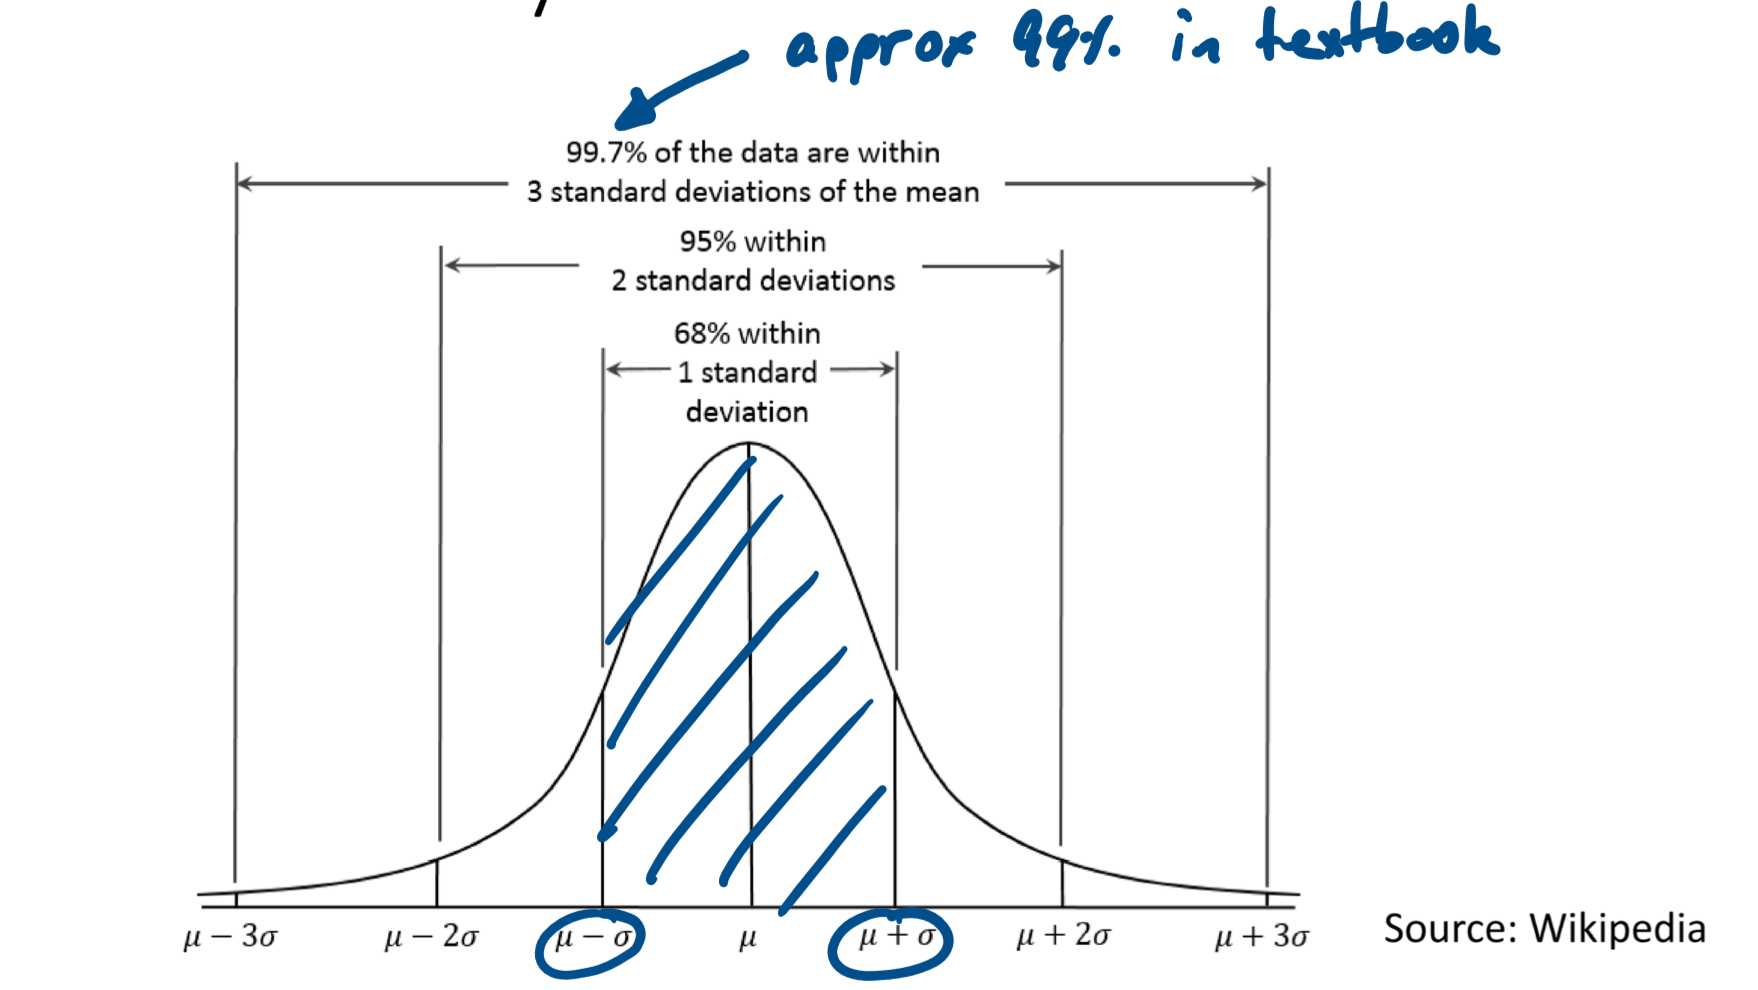
\includegraphics[width=\linewidth]{resources/ch5/normal-distribution-spread.png}
    \end{figure}
    
  \subsection{standard Normal Distribution}
    
\section{Standard Normal Distribution}

  For a continuous random variable $ X $ is normal if
  \begin{equation}
    p \left( x \right) = \frac{1}{\sqrt{2\pi}} \exp \left( -\frac{x^{2}}{2} \right)
  \end{equation}

  \begin{itemize}
    \item Standardized random variable by
    \begin{itemize}
      \item Subtracting mean, $ \mu $;
      \item Dividing standard deviation, $ \sigma $;
    \end{itemize}
  \end{itemize}

  \subsection{Properties}

    \begin{align}
      \E \left[ X \right] &= 0 \\
      \var \left[ X \right] &= 1
    \end{align}
    
\section{Central Limit Theorem}

  \begin{itemize}
    \item The distribution of the sum of $ N \to \infty $ \textbf{identically distributed (IID) random variables} is close to normal distribution;
    \begin{itemize}
      \item A binomial distribution is the \textbf{sum of IID bernouli random variables};
    \end{itemize}
  \end{itemize}
  
  \subsection{Normal Approximation}
  
    \begin{enumerate}
      \item Figure out the mean $ \mu $, which is the \textbf{expected value} (Refer to \ref{eq: ch4-expected-value-as-mean} on page \pageref{eq: ch4-expected-value-as-mean});
      \item Figure out the standard deivation $ \sigma $, which is \textbf{the square root of the variance} (Refer to \ref{eq: ch4-std-is-sqrt-var} on page \pageref{eq: ch4-std-is-sqrt-var});
      \item Plug $ \mu $ and $ \sigma $ into equation \ref{eq: ch5-normal-dist} on page \pageref{eq: ch5-normal-dist}, \textbf{integrate if needed};
    \end{enumerate}